\section{Experimental design}
\label{sec:experiments}

\subsection{Channel profiles and information budgets}
Table~\ref{tab:profiles} lists five controlled model profiles. The two dense
profiles test correctly specified integer subspaces with different power-delay
spreads, and the sparse integer profile examines the effect of sparsity without
fractional delays. The remaining profiles introduce separated fractional paths
and a closely spaced pair. These controlled profiles isolate delay geometry,
sparsity, and power spread rather than represent a standardized channel family.
All channel and noise draws are independent between Monte Carlo groups.
Within a group, 16 blocks share delays, powers, and noise variance. Their gains
are independent except in the correlation audit.

\begin{table}[t]
\centering
\caption{Simulated power-delay profiles. Delays are in base-rate sample periods;
all powers sum to one. The receiver is not given the profile identity or true
path count.}
\label{tab:profiles}
\small
\begin{tabular}{lll}
\toprule
Profile & Delays & Relative powers \\
\midrule
Exp-2 & $0,1,\ldots,11$ & $p_j\propto e^{-j/2}$ \\
Exp-8 & $0,1,\ldots,11$ & $p_j\propto e^{-j/8}$ \\
Sparse integer & $0,7,11$ & $0.5,0.3,0.2$ \\
Separated fractional & $0,7.35,11.2$ & $0.5,0.3,0.2$ \\
Close fractional & $0,3.1,3.45,10.7$ & $0.4,0.2,0.2,0.2$ \\
\bottomrule
\end{tabular}
\end{table}

Each target block contains 16 pilots at FFT indices $0,4,\ldots,60$ and 48 unit-energy
QPSK data symbols, with a CP of 16 base-rate samples. The noise variance is
$v=10^{-s/10}$ for nominal SNR $s\in\{0,10,20\}$~dB. Residual calibration
uses $T=1,4,$ or $16$ blocks with $d=4$. A separate control uses 64 independent
signal-free complex noise samples. These additional observations are counted
separately from the pilot budget. The CP control
uses four already transmitted repeated samples per block, together with the
useful-symbol samples and a known delay upper bound of 12. The known-noise
reference receives the true $v$; the oracle LMMSE reference also receives
the exact physical channel covariance. The practical controls fit the channel
using data from the target block alone.

\begin{table}[t]
\centering
\caption{Information resources of the numerical controls. Every channel estimate
uses the same target pilots within a paired comparison. Scalar pooling shares
noise statistics across blocks; it does not jointly fit their channel geometry.}
\label{tab:resources}
\small
\renewcommand{\arraystretch}{1.12}
\begin{tabular}{@{}>{\raggedright\arraybackslash}p{0.18\linewidth}>{\raggedright\arraybackslash}p{0.30\linewidth}>{\raggedright\arraybackslash}p{0.26\linewidth}>{\raggedright\arraybackslash}p{0.18\linewidth}@{}}
\toprule
Control & Calibration data and sharing & Supplied model information & Reported metric \\
\midrule
Residual & $T$ blocks of 16 pilots; residual energies pooled & Fixed integer
subspace; refined fit uses $[0,12]$ & Noise; full-channel NMSE/BER \\
Extended EB & 16 pilot blocks; one residual dimension per block & Integer
columns $-2,\ldots,12$ & Full-channel NMSE/BER \\
CP & Four CP--tail pairs per block, 16 blocks; energies pooled & Delay bound
12 and a clean repetition interval & Noise; full-channel NMSE/BER \\
Noise probes & 64 additional signal-free complex samples & Stationary noise
variance & Noise calibration \\
Known noise / oracle & True $v$; target pilots for channel estimation & Refined:
$[0,12]$; oracle: exact channel covariance & Full-channel NMSE/BER \\
VALSE & One target pilot block; joint noise and channel inference & Circular
frequency support; inferred order and noise & Noise; pilot-domain NMSE \\
\bottomrule
\end{tabular}
\end{table}

\subsection{Specified channel estimators}
Let $\mathbf F_L$ denote the response of integer delays $0,\ldots,L-1$ on
all subcarriers. The delay-domain least-squares estimate is
$\widehat{\mathbf H}=\mathbf F_L\mathbf z_1$. The main inexpensive control
uses positive-part empirical-Bayes (EB) shrinkage,
\begin{equation}
 \widehat h_\ell=z_{1,\ell}
 \left(1-\frac{\widehat v}{M|z_{1,\ell}|^2}\right)_+,
 \qquad \widehat{\mathbf H}=\mathbf F_L\widehat{\mathbf h},
 \label{eq:eb}
\end{equation}
with zero output when $z_{1,\ell}=0$. A cyclically extended control uses the
15 integer-delay columns $-2,\ldots,12$, leaving one residual complex
dimension per block. It uses the same shrinkage rule with its own 16-block
residual statistic, so the extension changes both representation and calibration.
Uniform Gaussian shrinkage and a fixed bank of exponential power-delay priors
are retained in the numerical archive as auxiliary controls. The main comparisons
use the EB rule defined above.

The sparse continuous-delay control is a generic OMP/variable-projection
implementation. It starts at order zero and selects each new atom from the grid
$\{0,0.25,\ldots,12\}$ by maximum residual correlation. It then solves for
complex gains by least squares and jointly refines all selected delays in $[0,12]$.
Variable projection eliminates the gains. The bounded dogbox optimizer uses an
analytic real-delay Jacobian and allows at most 60 objective evaluations per
candidate, with tolerances $10^{-9}$ for function/step changes and $10^{-10}$
for the gradient. Any refinement that increases the residual norm is rejected.
All visited orders, up to six paths, are compared using
\begin{equation}
 \mathrm{score}(k)=\frac{2\operatorname{RSS}_k}{\widehat v}
                  +d_k\log(2M),\qquad
 d_k=\begin{cases}2k,&\text{fixed-grid gains},\\3k,&\text{continuous delays and gains}.
 \end{cases}
 \label{eq:bic}
\end{equation}
The search can stop when the next order's penalty alone exceeds the current
minimum score. A scale-dependent numerical floor is used solely to avoid
division by zero. Equation~\eqref{eq:bic} is a BIC-type heuristic
with a supplied noise estimate; its finite-sample behavior depends on discrete
search multiplicity and path resolution. The grid
control omits continuous refinement and uses $d_k=2k$, so comparison with
the refined control changes both the fit and the parameter penalty.

The oracle reference is
\begin{equation}
 \widehat{\mathbf H}_{\rm or}=
 \mathbf C_{H,\mathcal P}
 (\mathbf C_{\mathcal P,\mathcal P}+v\mathbf I_M)^{-1}\mathbf y_1,
 \label{eq:oracle}
\end{equation}
where $\mathbf C_H$ is generated from the true delays and powers. This reference
quantifies the performance available with exact channel covariance and noise.

\subsection{Replication, metrics, and numerical validation}
\label{sec:reproducibility}
The broad calibration sweep uses three seeds with 5000 groups per cell
(15\,000 total). The full reconstruction sweep uses three different seeds with
300 groups per cell (900 total). The correlation audit uses 20\,000 groups
for each $\rho\in\{0,0.9,0.99,1\}$, with paired $T=1,4,16$ statistics.
These sweeps are exploratory. After inspecting them, we fixed two fractional
profiles, SNRs 10 and 20~dB, all estimator settings, and three new seeds for
a separate CP-control protocol. We then generated 300 groups per seed and cell,
without using the new observations for estimator tuning. Within each experiment,
all methods receive identical target channels, pilot noise, and data symbols.

Full-channel normalized mean-square error is computed from aggregate energies,
\begin{equation}
 \mathrm{NMSE}=\frac{\sum_{i=1}^{G}\|\widehat{\mathbf H}_i-\mathbf H_i\|^2}
                    {\sum_{i=1}^{G}\|\mathbf H_i\|^2}.
 \label{eq:nmse}
\end{equation}
Per-realization ratios are not averaged. Uncoded BER uses the signs
of the real and imaginary parts of $Y_k\widehat H_k^*$ on the 48 data tones,
giving 96 bits per target block. Bootstrap intervals are obtained by resampling
whole groups with the same indices for both methods. Positive gain denotes
$10\log_{10}(\mathrm{MSE}_{\rm reference}/\mathrm{MSE}_{\rm candidate})$.
The exploratory reconstruction intervals use 400 resamples; the independent
CP contrasts use 2000. These are pointwise percentile intervals without
multiplicity adjustment; bits within one fading realization are not treated
as independent bootstrap observations. We summarize noise calibration by
the mean ratio $\mathbb E[\widehat v]/v$ and the relative
standard deviation $\sqrt{\operatorname{Var}(\widehat v)}/v$, estimated across
groups. The relative standard deviation uses the true thermal variance as its
denominator rather than the potentially biased mean estimate.

The CP experiment generates independent frequency-domain Gaussian receiver
noise, transforms it by a unitary IFFT to obtain the useful-symbol tail,
and combines that tail with independent CP noise. The same frequency-domain
noise is used on pilots and data. This construction is equivalent to generating
white base-rate time noise and preserves the dependence in
\eqref{eq:cpdependence}. An independent check of signal cancellation uses
linear path shifts of a finite CP-extended waveform at oversampling factor
20. All delays in Table~\ref{tab:profiles} lie exactly on this oversampling
grid. In this audit, the fractional-delay and integer-delay FFT-response
discrepancies are below $9\times10^{-15}$. Shortening the CP to eight samples
produces a relative RMS discrepancy of 0.151 for the fractional example.
The four CP signal pairs also cancel to numerical precision in every profile.

Experiments use Python 3.13.9, NumPy 2.1.3, and SciPy 1.17.1 on CPU, with
one BLAS thread per process. No learned model or GPU training is used. Source
hashes, seeds, per-group errors, and optimizer diagnostics are retained. Numerical
tests check projection moments, variable-projection derivatives, noiseless
recovery, the CP control, and the variational implementation described below.
OpenAI Codex was used for debugging assistance.

\section{Results}
\label{sec:results}

\subsection{Averaging controls variance, not fractional-delay leakage}
Figure~\ref{fig:calibration} compares predicted and empirical calibration
statistics. The separated fractional profile has a projected signal bias
of $b=0.0777473$, giving an expected noise ratio at 20~dB of
$1+b/0.01=8.7747$. Across 15\,000 groups, the measured ratios for
$T=1,4,16$ are 8.754, 8.784, and 8.783, while their relative standard
deviations fall from 7.673 to 3.897 and 1.927. The matched Exp-2 profile has
a 16-block ratio of 1.0002 and relative standard deviation
0.1242, close to $1/\sqrt{64}=0.125$. The additional 64 independent noise
probes also give a ratio close to one. Finite noise-sample variance alone
therefore does not explain the discrepancy under fractional delays.

\begin{figure}[t]
\centering
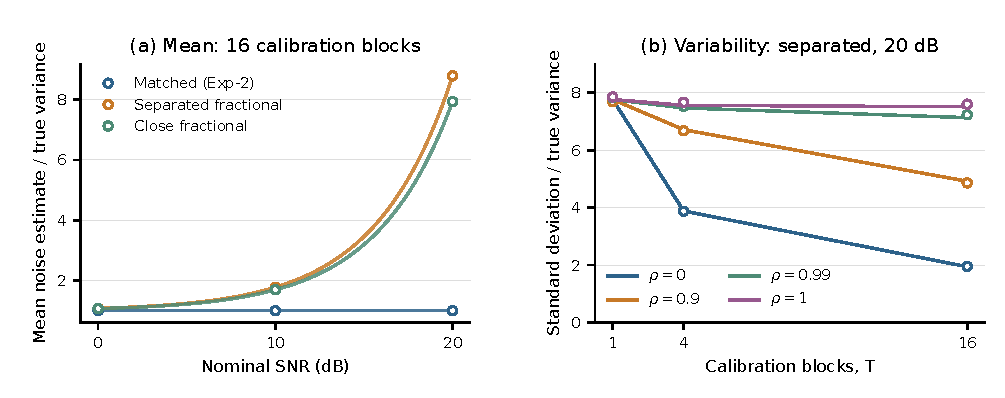
\includegraphics[width=\linewidth]{calibration_bias.pdf}
\caption{Residual-noise calibration. (a) Empirical 16-block means (markers,
15\,000 groups per condition) and analytical expectations (curves).
(b) Empirical relative standard deviations (markers, 20\,000 groups per
correlation condition) and Gaussian predictions (lines joining the evaluated
block counts), for the separated fractional profile at 20~dB. Correlation
acts on the leaked channel energy; the mean remains biased at every block count.}
\label{fig:calibration}
\end{figure}

The gain from pooling depends strongly on temporal correlation. In the separate
correlation audit, the measured relative standard deviation at $T=16$ is
1.955 for independent gains, 4.861 for $\rho=0.9$, 7.235 for $\rho=0.99$,
and 7.605 for constant gains. The corresponding analytical values are
1.942, 4.920, 7.135, and 7.513. The observations agree with the separate
receiver-noise and channel-leakage terms in \eqref{eq:varianceparts}.
Thus the benefit of a 16-block window depends on its temporal spacing and
gain correlation.

For the integer EB receiver, increasing residual pooling from one to 16 blocks
in the separated fractional 20~dB case improves NMSE by 0.047~dB
(pointwise 95\% interval [0.029, 0.064]~dB), while BER increases by 0.00067
(95\% interval [0.00050, 0.00083]).
A residual estimate can thus become sharply concentrated while a substantial
reconstruction error floor remains.

\subsection{Delay offset, subspace width, and useful averaging}
\label{sec:operatingregion}
A prespecified sensitivity study varies the pilot count, delay offset, and
integer-window length. It uses $N=64$, $M\in\{16,32\}$ equally spaced pilots,
delays $(0,7+\delta,11+\delta)$, powers $(0.5,0.3,0.2)$,
$\delta=0,0.1,\ldots,0.9$, and $L=12,13,14,15$.
The 160 combinations of geometry and SNR (10 and 20~dB) are evaluated
analytically for $T=1,4,16$. Independent Monte Carlo checks use 20\,000 groups
per condition at 20~dB for both pilot counts, $L=12,15$, and
$\delta=0,0.2,0.5,0.9$. The complete grid and group estimates are archived.

Figure~\ref{fig:operatingregion} shows how the crossover changes with the
channel geometry. Here normalized calibration MSE means
$\mathbb E[(\widehat v_T-v)^2]/v^2$, distinct from the full-channel NMSE in
Eq.~\eqref{eq:nmse}. At $M=16$, $\delta=0.5$, and 20~dB, increasing $L$ from
12 to 15 reduces $b/v$ from 40.79 to 5.00 and normalized calibration MSE
at $T=16$ from 1765.78 to 27.24. The corresponding $T_\star$ values are
0.98 and 1.44 blocks: both estimates are bias-dominated well before 16
independent blocks. With 32 pilots, the same window change reduces normalized
MSE from 333.46 to 7.31. Across the 48 Monte Carlo checks (16 conditions,
three block counts), means and mean-square errors differ from their predictions
by at most 2.91 and 2.79 Monte Carlo standard errors; sample variances differ
by at most 3.02\%.

\begin{figure}[t]
\centering
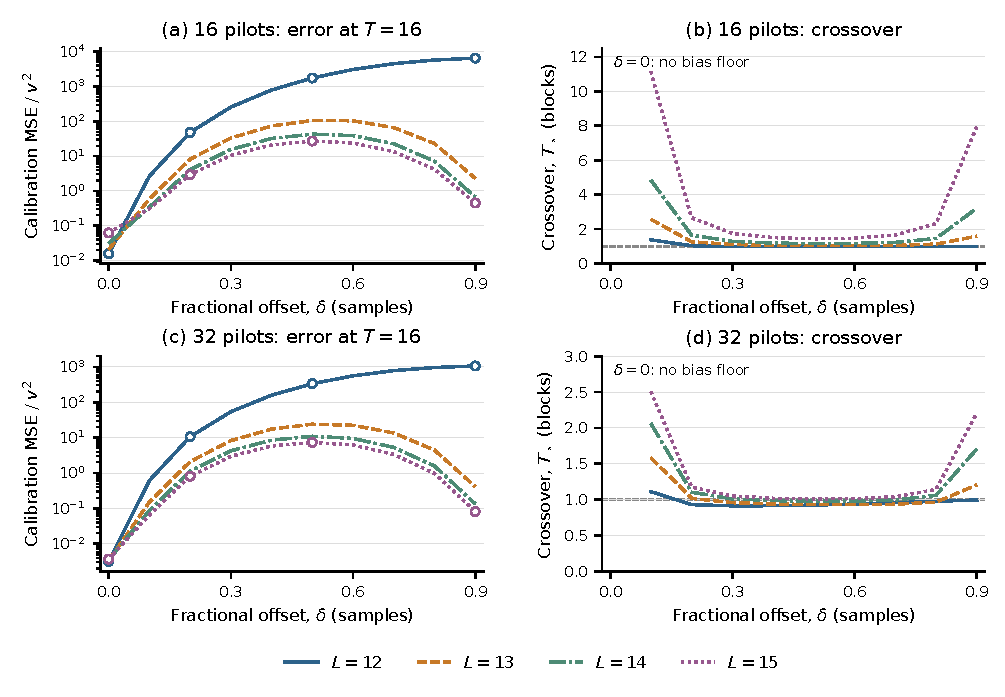
\includegraphics[width=\linewidth]{operating_region.pdf}
\caption{Geometry and window sensitivity at 20~dB with independent gains.
Left: normalized calibration MSE at $T=16$; curves give the analytical
grid and open circles the Monte Carlo checks for $L=12,15$ (20\,000 groups
per condition). Right: the bias--variance crossover $T_\star$ for nonzero
offsets. At $\delta=0$, the channel lies in every tested subspace and there
is no finite crossover. The dashed horizontal reference marks one block.
Lines connect evaluated offsets; the full archive also contains 10~dB and
$T=1,4$ results.}
\label{fig:operatingregion}
\end{figure}

Wider windows reduce both raw leakage and normalized bias at every fractional
offset in this grid, but the calibration MSE also depends on the remaining
residual dimensions. At $M=16$, $\delta=0.1$, and 10~dB, changing $L$ from
12 to 15 lowers $b/v$ from 0.157 to 0.043 while increasing normalized MSE
at $T=16$ from 0.0465 to 0.0698. The intermediate choice $L=13$ gives
0.0292, the smallest MSE among the four tested widths in this condition.
For the matched integer case, the same
change increases MSE from $1/64$ to $1/16$. Thus a wider window is beneficial
when the leakage reduction compensates for the variance cost. The crossover
and MSE quantify that trade-off for the specified channel family and noise level.


\subsection{Confirmation with cyclic-prefix calibration}
The paired CP experiment changes the received calibration samples while
keeping the receiver, its search settings, and the target channel and pilot
realization fixed. It uses the existing CP and its useful-symbol counterparts.
Figure~\ref{fig:cp} shows all four prespecified conditions. CP noise ratios range
from 0.9999 to 1.0069, with relative standard deviations 0.121--0.129,
consistent with the predicted value 0.125. At 20~dB, the corresponding
residual ratios are 8.781 and 7.882 for separated and close fractional paths.

\begin{figure}[t]
\centering
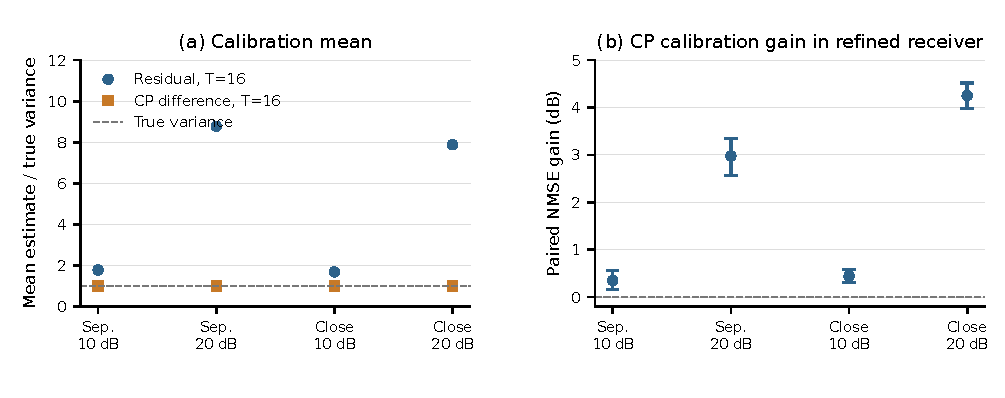
\includegraphics[width=\linewidth]{cp_confirmation.pdf}
\caption{Independent CP-control experiment: 900 groups per cell from three
new seeds. (a) Noise-calibration ratios. (b) NMSE gain obtained by replacing
16-block pilot-residual calibration with 16-block CP calibration in the
same refined receiver. Error bars are pointwise 95\% paired bootstrap
intervals from 2000 resamples. CP and FFT noise retain their physical dependence.}
\label{fig:cp}
\end{figure}

For separated paths at 20~dB, the refined receiver changes from $-21.76$~dB
with residual calibration to $-24.74$~dB with CP calibration; the paired
gain is 2.98~dB [2.57, 3.34]. For close paths, it changes from $-19.15$
to $-23.41$~dB, a gain of 4.25~dB [3.97, 4.52]. BER changes from 0.01000
to 0.00662 and from 0.01206 to 0.00756, respectively. The remaining NMSE
differences from the known-noise controls are 0.10 and 0.04~dB. At 10~dB,
CP gains are smaller, 0.35~dB [0.16, 0.56] and 0.44~dB [0.30, 0.59],
consistent with the smaller leakage-to-noise ratio.

The integer EB receiver gains 0.82 and 0.84~dB at 20~dB on the
same observations. Its CP-calibrated NMSE remains $-13.93$ and $-13.66$~dB.
The smaller gain leaves a substantial representation-dependent error.
In the continuous receiver, the mean selected order
rises from 2.73 to 3.11 for separated paths and from 2.99 to 3.86 for close
paths when CP calibration replaces residual calibration. The changes are
consistent with the residual estimate suppressing weaker components through
the score in \eqref{eq:bic}. These statistics describe the selected orders
as receiver decisions rather than estimates of an exactly identified path count.

The main calibration contrast is stable under an increased optimization
budget: rerunning the flagged fits changes each primary 20~dB CP gain by less
than $10^{-4}$~dB. The original setting selected a candidate at its evaluation
limit in 121 of 10\,800 refined fits; four such cases remained after the budget
extensions. Appendix~\ref{app:optimizer} gives the full diagnostic counts.

\subsection{Representation and calibration have distinct effects}
Figure~\ref{fig:reconstruction} and Table~\ref{tab:reconstruction} compare the
controls for full-channel reconstruction. In the separated fractional 20~dB
case, extending the integer window improves NMSE from $-13.11$ to $-14.43$~dB. Continuous-delay
fitting with the original pooled residual statistic reaches $-22.36$~dB,
a paired gain of 7.93~dB over the extended EB control (95\% interval
[7.54, 8.38]~dB). Supplying the true noise variance to the same continuous
receiver improves NMSE further to $-25.07$~dB. Changing the representation
removes much of the error, but contaminated calibration still affects
model-order selection.

\begin{figure}[t]
\centering
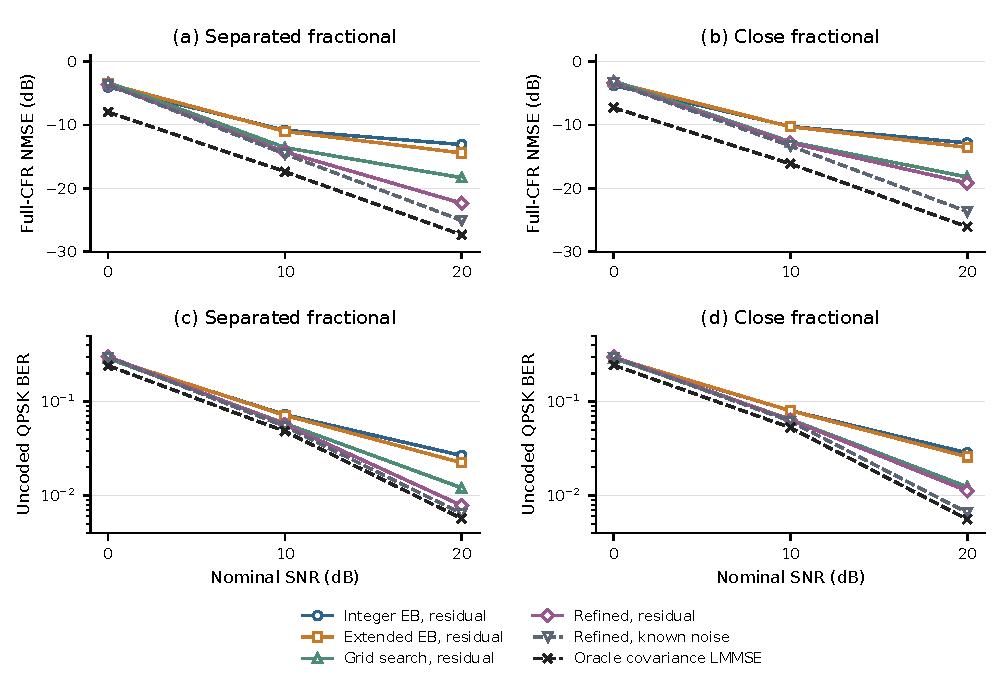
\includegraphics[width=\linewidth]{reconstruction.pdf}
\caption{Exploratory full-channel reconstruction and uncoded detection with
900 paired groups per cell. Residual controls use 16 calibration blocks;
the extended integer control computes its own one-dimensional residual.
The grid and refined controls have different order penalties. Known noise
and exact-covariance LMMSE are explicitly identified information-rich references.}
\label{fig:reconstruction}
\end{figure}

\begin{table}[t]
\centering
\caption{Full-channel NMSE (dB) at 20~dB nominal SNR; 900 paired groups per profile. Integer EB, extended EB, and grid/refined residual controls use 16-block calibration. The known-noise and oracle columns receive extra statistical information.}
\label{tab:reconstruction}
\small\setlength{\tabcolsep}{4pt}
\begin{tabular}{lrrrrrr}
\toprule
& Integer & Extended & Grid & Refined & Refined & Oracle \\
Profile & EB & EB & residual & residual & known $v$ & LMMSE \\
\midrule
Exp-2 & -21.16 & -20.91 & -13.65 & -15.55 & -15.55 & -21.54 \\
Exp-8 & -21.13 & -20.88 & -9.09 & -9.94 & -9.94 & -21.29 \\
Sparse integer & -25.25 & -24.66 & -24.87 & -25.28 & -25.31 & -27.57 \\
Separated fractional & -13.11 & -14.43 & -18.34 & -22.36 & -25.07 & -27.35 \\
Close fractional & -12.84 & -13.55 & -18.23 & -19.19 & -23.67 & -26.06 \\
\bottomrule
\end{tabular}
\end{table}

The gap is larger for the closely spaced profile, where the refined residual
control gives $-19.19$~dB and the known-noise version $-23.67$~dB.
The dense profiles favor the integer subspace. The six-path refined control
gives $-15.55$ and $-9.94$~dB for Exp-2 and Exp-8, whereas integer EB gives
$-21.16$ and $-21.13$~dB. The path cap is below the 12 generating paths in
these cases. The dense-profile comparison is therefore specific to this
six-path fit and its selection and optimization settings. Continuous-delay models can also represent dense
channels through a richer virtual channel impulse response, as demonstrated
by Hansen et al.\ \cite{hansen2018iterative}.

\subsection{Joint inference with a continuous probabilistic model}
Joint continuous-parameter inference provides a second route to separating
signal and noise. We evaluate a Python implementation of VALSE Heuristic~2
from the paper equations \cite{badiu2017valse}, retaining frequency and gain
uncertainty in the noise update. VALSE learns from one target block over a
circular frequency support, while the refined control uses the delay bound
$[0,12]$ and 16 calibration blocks for its residual statistic. The comparison
therefore measures pilot-domain reconstruction and inferred noise under these
different resources. Full-channel interpolation would additionally require a
physical delay branch for the frequency posterior.

Three new seeds give 450 paired groups for each of three sparse profiles
at 10 and 20~dB. The primary setting uses a 500-iteration limit and a relative
reconstruction-change tolerance of $10^{-6}$. All 2700 outputs are retained:
2688 met the stopping criterion, and 12 reached the iteration limit.
Appendix~\ref{app:valse} details the implementation and numerical checks.
Replaying the 12 capped inputs with a 5000-iteration ceiling gives 11 further
convergences. Across the six cells, pilot NMSE changes by at most
0.000624~dB and the mean inferred-noise ratio by $2.72\times10^{-5}$.
The primary table retains the original 500-iteration outputs.

\begin{table}[t]
\centering
\caption{Pilot-domain reconstruction and noise inference; 450 groups per cell. Columns 3--6 give NMSE in dB. VALSE learns noise from one block with circular frequency support; refined controls use the delay bound $[0,12]$. The comparison concerns the observed pilot grid.}
\label{tab:valse}
\small\setlength{\tabcolsep}{4pt}
\begin{tabular}{lrrrrrr}
\toprule
& SNR & Integer & Refined & Refined & VALSE & VALSE \\
Profile & (dB) & EB & residual & known $v$ & & $\mathbb E[\widehat v]/v$ \\
\midrule
Sparse integer & 10 & -14.86 & -14.44 & -14.55 & -14.30 & 1.04 \\
Sparse integer & 20 & -24.98 & -24.86 & -24.86 & -23.86 & 1.13 \\
Separated fractional & 10 & -10.95 & -14.09 & -14.57 & -14.46 & 1.04 \\
Separated fractional & 20 & -13.76 & -22.13 & -24.97 & -23.92 & 1.17 \\
Close fractional & 10 & -10.75 & -12.76 & -13.24 & -12.97 & 1.12 \\
Close fractional & 20 & -13.82 & -18.92 & -23.83 & -19.85 & 1.94 \\
\bottomrule
\end{tabular}
\end{table}

Table~\ref{tab:valse} shows noise inference with a continuous probabilistic
model. At 20~dB, the mean noise ratios were 1.13, 1.17, and 1.94 for integer,
separated fractional, and close fractional paths, respectively. The larger
close-pair ratio accompanies a larger pilot reconstruction error, identifying
a condition where the specified joint inference retains appreciable calibration
error. For separated fractional paths, pilot NMSE was $-23.92$~dB,
between the residual-calibrated and known-noise refined controls. These
pilot-domain observations complement the full-channel CP intervention by
showing how calibration also depends on the inferential model.

